\documentclass[fleqn,10pt]{latex/stylish_article} % Document font size and equations flushed left

\setcounter{tocdepth}{3}

% Pandoc environments
\usepackage{framed}
\usepackage{fancyvrb}
\providecommand{\tightlist}{%
  \setlength{\itemsep}{0pt}\setlength{\parskip}{0pt}}
\newcommand{\VerbBar}{|}
\newcommand{\VERB}{\Verb[commandchars=\\\{\}]}
\DefineVerbatimEnvironment{Highlighting}{Verbatim}{commandchars=\\\{\}, fontsize=\scriptsize} % R Code

% Colored code
\usepackage{color}
\definecolor{shadecolor}{RGB}{248,248,248}
\newenvironment{Shaded}{\begin{snugshade}}{\end{snugshade}}
\newcommand{\KeywordTok}[1]{\textcolor[rgb]{0.13,0.29,0.53}{\textbf{{#1}}}}
\newcommand{\DataTypeTok}[1]{\textcolor[rgb]{0.13,0.29,0.53}{{#1}}}
\newcommand{\DecValTok}[1]{\textcolor[rgb]{0.00,0.00,0.81}{{#1}}}
\newcommand{\BaseNTok}[1]{\textcolor[rgb]{0.00,0.00,0.81}{{#1}}}
\newcommand{\FloatTok}[1]{\textcolor[rgb]{0.00,0.00,0.81}{{#1}}}
\newcommand{\ConstantTok}[1]{\textcolor[rgb]{0.00,0.00,0.00}{{#1}}}
\newcommand{\CharTok}[1]{\textcolor[rgb]{0.31,0.60,0.02}{{#1}}}
\newcommand{\SpecialCharTok}[1]{\textcolor[rgb]{0.00,0.00,0.00}{{#1}}}
\newcommand{\StringTok}[1]{\textcolor[rgb]{0.31,0.60,0.02}{{#1}}}
\newcommand{\VerbatimStringTok}[1]{\textcolor[rgb]{0.31,0.60,0.02}{{#1}}}
\newcommand{\SpecialStringTok}[1]{\textcolor[rgb]{0.31,0.60,0.02}{{#1}}}
\newcommand{\ImportTok}[1]{{#1}}
\newcommand{\CommentTok}[1]{\textcolor[rgb]{0.56,0.35,0.01}{\textit{{#1}}}}
\newcommand{\DocumentationTok}[1]{\textcolor[rgb]{0.56,0.35,0.01}{\textbf{\textit{{#1}}}}}
\newcommand{\AnnotationTok}[1]{\textcolor[rgb]{0.56,0.35,0.01}{\textbf{\textit{{#1}}}}}
\newcommand{\CommentVarTok}[1]{\textcolor[rgb]{0.56,0.35,0.01}{\textbf{\textit{{#1}}}}}
\newcommand{\OtherTok}[1]{\textcolor[rgb]{0.56,0.35,0.01}{{#1}}}
\newcommand{\FunctionTok}[1]{\textcolor[rgb]{0.00,0.00,0.00}{{#1}}}
\newcommand{\VariableTok}[1]{\textcolor[rgb]{0.00,0.00,0.00}{{#1}}}
\newcommand{\ControlFlowTok}[1]{\textcolor[rgb]{0.13,0.29,0.53}{\textbf{{#1}}}}
\newcommand{\OperatorTok}[1]{\textcolor[rgb]{0.81,0.36,0.00}{\textbf{{#1}}}}
\newcommand{\BuiltInTok}[1]{{#1}}
\newcommand{\ExtensionTok}[1]{{#1}}
\newcommand{\PreprocessorTok}[1]{\textcolor[rgb]{0.56,0.35,0.01}{\textit{{#1}}}}
\newcommand{\AttributeTok}[1]{\textcolor[rgb]{0.77,0.63,0.00}{{#1}}}
\newcommand{\RegionMarkerTok}[1]{{#1}}
\newcommand{\InformationTok}[1]{\textcolor[rgb]{0.56,0.35,0.01}{\textbf{\textit{{#1}}}}}
\newcommand{\WarningTok}[1]{\textcolor[rgb]{0.56,0.35,0.01}{\textbf{\textit{{#1}}}}}
\newcommand{\AlertTok}[1]{\textcolor[rgb]{0.94,0.16,0.16}{{#1}}}
\newcommand{\ErrorTok}[1]{\textcolor[rgb]{0.64,0.00,0.00}{\textbf{{#1}}}}
\newcommand{\NormalTok}[1]{{#1}}

% cslreferences environment required by pandoc > 2.7

% Polyglossia
\usepackage{polyglossia}
\setmainlanguage{en-US}
\setotherlanguage{fr-FR}
\setotherlanguage{it}

% localized quotes
\usepackage[strict,autostyle]{csquotes}

% Figures
\usepackage{graphicx,grffile}
\makeatletter
\def\maxwidth{\ifdim\Gin@nat@width>\linewidth\linewidth\else\Gin@nat@width\fi}
\def\maxheight{\ifdim\Gin@nat@height>\textheight0.8\textheight\else\Gin@nat@height\fi}
\makeatother
% Scale images if necessary, so that they will not overflow the page
% margins by default, and it is still possible to overwrite the defaults
% using explicit options in \includegraphics[width, height, ...]{}
\setkeys{Gin}{width=\maxwidth,height=\maxheight,keepaspectratio}

% Additional packages
\usepackage{natbib}             % Advanced Bibliography (citep...).
\usepackage{amsmath,amsfonts,amssymb}
\usepackage{breqn}              % Line breaks in equations
\usepackage{url}                % Line breaks in url's
\usepackage{enumitem}           % Line spacing in lists
  \setlist[itemize]{noitemsep,nolistsep}
  \setlist[enumerate]{noitemsep,nolistsep}

% Tables
\usepackage{longtable,booktabs}
\usepackage{caption}
% These lines are needed to make table captions work with longtable:
\makeatletter
\def\fnum@table{\tablename~\thetable}
\makeatother
% longtable 2 columns
% https://tex.stackexchange.com/questions/161431/how-to-solve-longtable-is-not-in-1-column-mode-error
\makeatletter
\let\oldlt\longtable
\let\endoldlt\endlongtable
\def\longtable{\@ifnextchar[\longtable@i \longtable@ii}
\def\longtable@i[#1]{\begin{figure}[t]
\onecolumn
\begin{minipage}{0.5\textwidth}\scriptsize
\oldlt[#1]
}
\def\longtable@ii{\begin{figure}[t]
\onecolumn
\begin{minipage}{0.5\textwidth}\scriptsize
\oldlt
}
\def\endlongtable{\endoldlt
\end{minipage}
\twocolumn
\end{figure}}
\makeatother

% Full-width tables
\usepackage{tabu}
\renewenvironment{table}{\begin{table*}}{\end{table*}\ignorespacesafterend}

% Prevent overfull lines
\setlength{\emergencystretch}{3em}

% User-adder preamble
\hyphenation{bio-di-ver-si-ty sap-lings}

% hyperref comes last
\usepackage{hyperref}           % Hypertext links, PDF bookmarks
  \hypersetup{%
    %
    linkcolor=black,citecolor=black,colorlinks=true%
  }

%----------------------------------------------------------------------------------------
%	ARTICLE INFORMATION
%----------------------------------------------------------------------------------------

\JournalInfo{Publication reference} % Journal information
\Archive{DOI: xxx/xx} % Additional notes (e.g. copyright, DOI, review/research article)

\PaperTitle{Title of the Article} % Article title

\Authors{
First Author's name\textsuperscript{1*}\\ Second Author's name\textsuperscript{2}
} % Authors
\affiliation{
\textsuperscript{1}Department / University\\ \hspace{1em} Street address, Zip code, Country.\\\textsuperscript{2}Department / University\\ \hspace{1em} Street address, Zip code, Country.
}
\affiliation{*\textbf{Corresponding author}: \href{mailto:name@company.com}{\nolinkurl{name@company.com}}, \url{https://www.company.com}} % Corresponding author

\Keywords{root vertical density, tropical forest structure, drainage, drought} % Keywords
\newcommand{\keywordname}{Keywords} % Defines the keywords heading name

%----------------------------------------------------------------------------------------
%	ABSTRACT
%----------------------------------------------------------------------------------------

\Abstract{
This study investigates the impact of drainage barriers on tree root distribution and forest structure in Paracou, French Guiana. Using the depth at which a horizon high in silt (HSD, high silt depth) occurs as a proxy for drainage barrier, the study explores the relationship between drainage barriers, topography, and forest community structure. Despite expectations of reduced root density in soil horizons with high silt content, no significant reduction of root density was found. Species richness and tree density showed a slight but significant decrease with increasing HSD, while diameter at breast height (DBH) exhibited minimal variation. The strong association between silt and mica content suggests the potential use of mica as a practical proxy for silt in future studies, streamlining data collection. These findings contribute valuable insights into the complexity of soil-root interactions in tropical ecosystems. Further research with increased sampling density and direct data collection is recommended to refine and expand upon these initial observations.
}

%----------------------------------------------------------------------------------------

\begin{document}

\selectlanguage{en-US}

\flushbottom % Makes all text pages the same height

\maketitle % Print the title and abstract box

\tableofcontents % Print the contents section

\thispagestyle{empty} % Removes page numbering from the first page

%----------------------------------------------------------------------------------------
%	ARTICLE CONTENTS
%----------------------------------------------------------------------------------------

\hypertarget{introduction}{%
\section{Introduction}\label{introduction}}

In tropical ecology, the relationship between root distribution and soil abiotic factors is crucial to forest community structure (Bardgett et al., 2014; Schlesinger, 1991). Roots are essential for the nutrition and water uptake of trees (Hodge, 2009; Hutchings et al., 2003). Root distribution is driven by factors like soil texture, nutrient content, topography, and water content (Freschet, 2021).
French Guiana features a topography alternating between hills and valleys (Ferry, 2003). Superficial lateral drainage (SLD) is the typical drainage type on slopes (Fan et al.~2017). SLD is characterised by a silty-clay texture horizon with low permeability that therefore functions as a drainage barrier in the soil (Ferry, 2003; Humbel, 1978). Drainage type, and to a lesser extent topography, are the main factors influencing forest community structure (Pélissier et al., 2002; Sabatier et al., 1997).
Root vertical distribution (RVD) is the distribution of roots in units of biomass over sequential soil layers (Freschet et al., 2021). The early appearing drainage barrier inhibits the vertical root development (Ferry et al., 2003; Pélissier et al., 2002). Soils with SLD have a small water reserve. Consequently, roots in this soil type may undergo drought stress during the dry season. During the rainy season, this impermeable layer will cause a temporal water table in the soil (Humbel, 1978; Pélissier et al., 2002), which creates anoxic stress to tree roots. Tree roots are therefore concentrated in the uppermost layers of the soil under SLD (Humbel, 1978).
Our study takes place at the Paracou research station in French Guiana. Epron (2006) confirmed the presence of SLD in this area. They found that the depth of the drainage barrier on slopes depended on the topographical position, with deeper barriers at higher elevation. However, the specific ways in which drainage barriers influence both roots and forest structure remain understudied. Therefore, we examined whether drainage barriers restrict tree roots on slopes in Paracou, exploring their role in shaping forest community structure. We use the depth at which silt appears in high concentration (HSD), and the mica content, as an indicator proxy of drainage barrier. We study the effect of the drainage barrier occurrence (HSD) on 3 different forest structure indicators (DBH, species richness and tree density) and on RVD . Our main hypotheses are that (1) root density is reduced when HSD appears closer to the surface and (2) HSD can be a predictor of DBH, species richness and tree density.

\hypertarget{material-and-method}{%
\section{Material and method}\label{material-and-method}}

\hypertarget{study-site}{%
\subsection{Study site}\label{study-site}}

The study took place at Paracou research station in French Guiana (5°18'N; 52°53'W), a 40 000 ha domain owned by CNES (National Centre for Space Studies) containing 16 permanent plots studied by the French research centre CIRAD for over 35 years . Elevation ranges from 5 to 50 m, and the mean annual temperature is 26 °C, with an annual range of 1--1.5 °C. Rainfall averages 2980 mm per year with a 3-month dry season (\textless{} 100 mm month) from mid-August to mid-November. The landscape is characterized by a patchwork of low hills (100--300 m wide and 20--35 m high) separated by narrow streams. The soil type in this area is mostly Acrisol and soil depth is restricted by a poorly draining, loamy saprolite, typically encountered at a depth of around 1 m (Epron et al.~2006).
Sampling was carried out as part of the ALT-project (Amazonian Landscapes in Transition 2022-2025).

\hypertarget{pit-data-collection}{%
\subsection{Pit data collection}\label{pit-data-collection}}

Pit excavation allows the collection of root distribution data (Freschet et al., 2021). Four pits were sampled between September 11 and 16, 2023, just outside of plot 16, next to the subplots 23-25, to avoid disturbances on inventoried trees.

All pits were excavated on mid-slope position, characterised by SLD. Potential pits were prospected using an auger to locate sites with different HSD, in order to diagnose the effect of silt on root development. Rectangular pits, 100 cm deep and 50 cm wide, were dug with pickaxes and spades.

After cleaning the exposed soil surface in the pits by scraping, colour and texture changes were used to identify horizons on one side of the pit (Ferry et al., 2003). The depth of each horizon was measured. Mica content and texture class were estimated. Soil samples were moistened to analyse the texture by touch (Jahn et al., 2006), using Jamagne's (1977) soil texture triangle. For two sides of the pit, we counted the roots using a 100 x 50 cm grid, subdivided in squares of 10 x 10 cm (Freschet et al., 2021). In each square, roots were counted and classified by diameter (\(< 2\) mm, \(2-5\) mm, \(5-10\) mm and \(≥ 10\) mm).

\hypertarget{auger-and-botanical-data}{%
\subsection{Auger and botanical data}\label{auger-and-botanical-data}}

In addition to our pit data, we used 36 auger samples collected during a 2022 data collection campaign on the P16 of Paracou, in the subplots 14, 15, 19 and 20 (Appendix 1 Fig. 1). In contrast to the pit data collection, root abundance was not sampled. For the complete auger collection method, we refer to Dogny Piette and Corbera Serrajorada (2022).
The botanical data corresponds to the 2020 inventory of the GUYAFOR tree database, which monitors trees of diameter at Breast Height (DBH) superior to 10 cm. In our study area, this data was completed with data from the ALT project, which also included trees of \(DBH > 1\) cm.

\hypertarget{data-analysis}{%
\subsection{Data analysis}\label{data-analysis}}

\hypertarget{pit-data-analysis}{%
\subsubsection{Pit data analysis}\label{pit-data-analysis}}

As for the auger data, soil textures in the pits were grouped into \enquote{high}, \enquote{intermediate}, and \enquote{low} silt content. Given the small sample size (4 pits), we chose to only conduct a visual analysis, concentrating on discernible tendencies. As roots were counted per layer of 10 cm, and soil texture was determined per soil horizon, we assigned a texture class to every 10 cm of the soil.
Root index was calculated by weighting each root count with its corresponding maximum diameter class. We then assessed the relation between root index and silt content. Root index was compared between pits for a specific depth range to account for the effect that root index decreases exponentially with depth.

\hypertarget{auger-and-botanical-data-analysis}{%
\subsubsection{Auger and botanical data analysis}\label{auger-and-botanical-data-analysis}}

Out of the 36 auger measurements available, we focused our analysis on the subset of 29 measurements that included texture class data. The auger points were located using the coordinates of the closest inventoried tree on the plot. We regrouped the soil textures into a categorial variable \enquote{silt content}, based on silt content deducted from the texture triangle (Jamagne, 1977): low (A, Alo, AS), intermediate (SL, SA, S), and high (LSA, LAS, LS). We defined the depth (cm) at which the silt content changed to high for each auger sample, which we refer to as \enquote{high silt depth} (HSD). HSD is used to indicate the depth of the drainage barrier, which has a silty-clay texture (Ferry, 2002; Humbel, 1978). For auger points without any horizons high in silt, we defined a depth of 100 cm, which is the maximum depth of the auger measurements. As topography, besides drainage type, strongly influences forest community structure (Baldeck et al.~2013), we did a correlation test (Spearman method due to non-normality of HSD) between elevation (m) and HSD (cm).
We map the area where auger samples were taken and created contour lines based on the values of HSD of the different auger points (Appendix 1, Fig. 2). The contour lines were created with the Contour Plugin in QGIS. We employed 10 cm contour line intervals, resulting in the formation of seven distinct HSD classes, spanning depths from 40 cm to 100 cm. With this approach, we successfully interpolated HSD values spatially across nearly the entire 4-ha study area. Every tree on the map could therefore be linked to a certain HSD class and the corresponding coverage area of each HSD class was also determined.
Species richness and total number of trees per HSD class were calculated for the trees on slopes. Due to the ordinal nature of the different HSD classes, they cannot be considered as a categorical variable in an Anova test. Hence, we assigned a specific intermediate HSD value to each HSD class; for example, an HSD class ranging from 40 to 50 cm was designated the value of 45. This creates a continuous HSD-value, allowing us to perform a Poisson regression for both species richness and number of trees (HSD continuous values as predictor, species richness or number of trees as response, offset= log(area per HSD class) ). The area The relationship between DBH and HSD did not show a distinct linear dependency (Fig. 1c and 1d), making it difficult to construct a precise model.
Muscovite (white mica) degrades into kaolinite (Nicolini et al.~2009) with a particle size classified as silts. Thus, to complement our detection of the drainage barrier, we try to use mica content as a complementary proxy of silt content. A chi-squared test was done to quantitatively assess the association between silt content (categorical variable) and mica content (categorical variable) in the different horizons of the auger data.

All analyses were performed in R (version 4.2.2) (R Core Team (2022). R: A language and environment for statistical computing. R Foundation for Statistical Computing, Vienna, Austria. URL \url{https://www.R-project.org/}) and QGIS (version 3.28 Firenze).

\hypertarget{results}{%
\section{Results}\label{results}}

\scriptsize

\normalsize
\#\# Pit data

In contrast to our expectations, the four pits show similar root index variations with depth, regardless the variation in silt content. Focussing on the specific depth range of 60-80 cm, it becomes evident that P3 (pit 3) root index exceeds that of P2 (pit 2), even though P3 shows high silt content and P2 intermediate silt content. A similar observation is made when using mica content as a proxy of silt content. Figure 1b shows a general decrease of root index with depth, from 60 roots at a depth of 10 cm to 10 roots at 50 cm.



\scriptsize

\begin{figure*}

{\centering 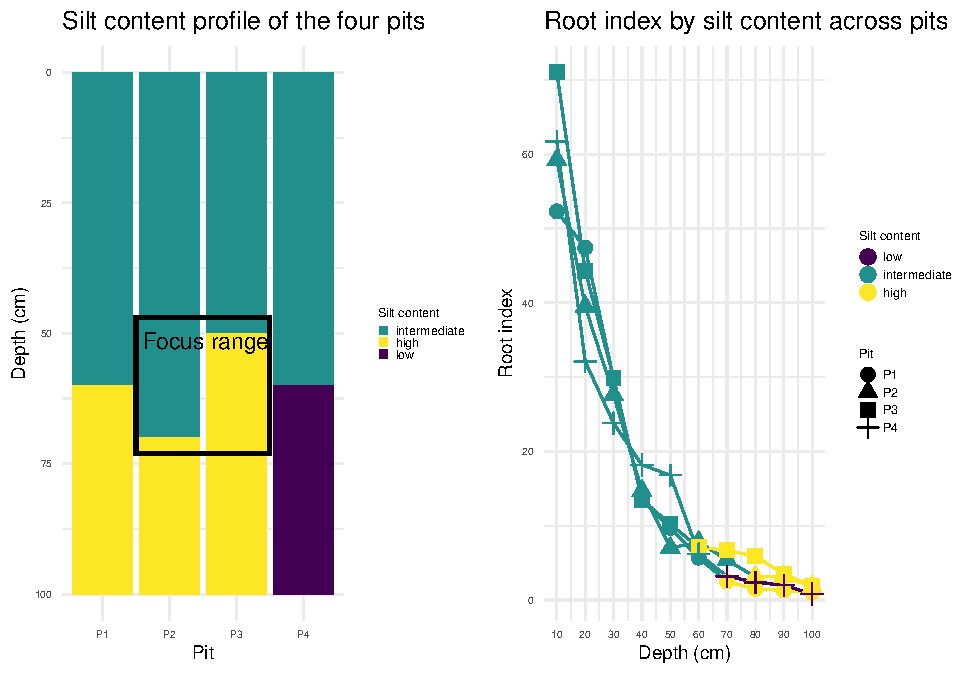
\includegraphics[width=0.8\linewidth,]{pedoP16-report_files/figure-latex/pit-1} 

}

\caption{a) Silt content and b) root index across pits excavated in September 2023. F1-4 correspond to pits 1-4.}\label{fig:pit}
\end{figure*}

\normalsize

\hypertarget{auger-data}{%
\subsection{Auger data}\label{auger-data}}

A significant negative correlation was found between elevation (m) and HSD (cm) (rho = - 0,634; p-value = 0.0002246). A higher position along the topographical gradient therefore indicates lower HSD.

Among all HSD classes, the range of 40 to 50 cm stands out with notably higher species richness (figure \ref{fig:auger}). This range contains the uppermost observed HSD. A significant but small decrease (p-value = 0.00245; Estimate = -0.0044) in species richness with HSD class can be observed (see Fig. 2a). Species richness and tree density is lowest for the 90 to 100 cm HSD range. For areas with no horizon high in silt, species richness was higher than for the HSD classes 70-100 cm, but lower than for horizons where silt appears closer to the surface. Tree density also significantly decreases with HSD class (p-value \textless{} 2e-16; Estimate = -0.013), although there is still an increase visible for the first HSD classes in the plot (see Fig. 2b). Samples without horizons high in silt show very low tree density of less than 5000 trees per ha.
Fig. 2c and 2d illustrate the relationship between the DBH and HSD classes. The mean DBH values and quantiles are very similar over all classes, only a small pattern is visible in the maximum value of the outliers, which increases with the HSD class.



\scriptsize

\begin{figure*}

{\centering 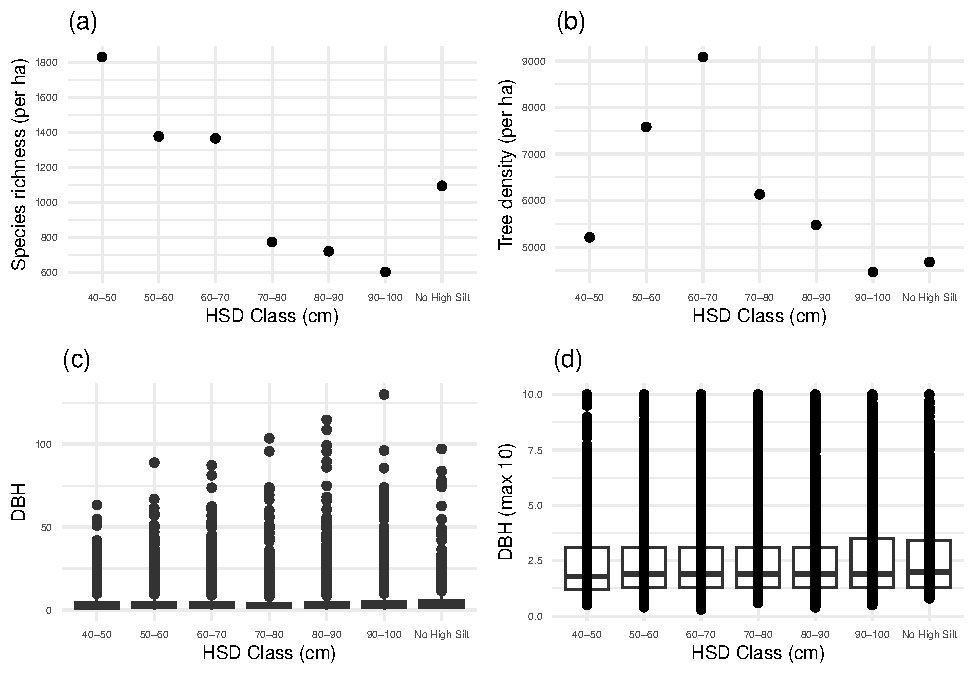
\includegraphics[width=0.8\linewidth,]{pedoP16-report_files/figure-latex/auger-1} 

}

\caption{Forest structure indicators relation with HSD (high silt depth) class. a) Species richness (per ha) in function of HSD classes, b) Tree density (per ha) in function of HSD classes, c) DBH (diameter at breast height) in function of HSD classes, d) DBH filtered (max value = 10 cm) in function of HSD classes}\label{fig:auger}
\end{figure*}

\normalsize
Figure 2 Forest structure indicators relation with HSD (high silt depth) class. a) Species richness (per ha) in function of HSD classes, b) Tree density (per ha) in function of HSD classes, c) DBH (diameter at breast height) in function of HSD classes, d) DBH filtered (max value = 10 cm) in function of HSD classes

\hypertarget{mica-as-a-proxy-for-silt}{%
\subsection{Mica as a proxy for silt}\label{mica-as-a-proxy-for-silt}}

The chi-squared test assessing the association between silt and mica content in the auger samples was highly significant (χ² = 49.994, df = 6, p = 4.715e-09). Cramer's V was 0.574, supporting a strong positive association. The Kruskal-Wallis showed a similar significance (χ² = 39.456, df = 2, p = 2.706e-09) and a Kruskal's τ(x,y)= 0.561, 0.231, which also confirms a strong association. The association is depicted in a mosaic plot in Appendix 2 (Fig. 1). illustrating an increase of silt content with rising mica content.

\hypertarget{discussion}{%
\section{Discussion}\label{discussion}}

\hypertarget{root-distribution-with-hsd-and-depth}{%
\subsection{Root distribution with HSD and depth}\label{root-distribution-with-hsd-and-depth}}

Our findings align with literature, illustrating that most roots are present within the first 30 cm of the soil (Freshet, 2021; Schenk and Jackson, 2002). HSD range across the pits, spanning from 50 cm to 70 cm (Fig. 1a), coincides with the depth range (60-80 cm) of the drainage barrier identified by Epron et al.~(2006).

We expected the HSD to act as a barrier for roots, and therefore to find less roots below the HSD, as was observed by Humbel (1978). However, there is no discernible effect of HSD on the vertical root distribution (Fig. 1b), no matter the root diameter observed (Appendix 2 Fig. 2). Roots of certain species can penetrate the drainage barrier and might be adapted to the drought constraints this can pose (Ferry, 2003). The absence of an observed effect may also be due to the narrow depth range of 20 cm, within which the two pits exhibited differences in silt content. Additionally, the restricted sample size of 4 pits precluded the performance of a statistical test. More soil pits would be needed to study root distribution in additional soil profiles. However, soil pit profiles are a very time-consuming and destructive method, despite the essential insights they provide for root and soil analysis.

\hypertarget{predicting-forest-structure-indicators-with-hsd}{%
\subsection{Predicting forest structure indicators with HSD}\label{predicting-forest-structure-indicators-with-hsd}}

No linear dependency was found between HSD and DBH measurements (Fig. 2c). The mean DBH values appear consistent over all HSD classes (Fig. 2d). A trend can be observed in the outliers per class, where the maximum DBH value increases with HSD class. This observation might indicate that trees can achieve a larger DBH in soils with fewer drainage restrictions.
As DBH did not vary significantly between different HSD classes, tree density variation indirectly indicates variations in basal area. We found a significant negative effect of HSD on density, with a maximum tree density per ha observed at a medium HSD between 60 and 70 cm. This indicates that as the drainage barrier is closer to the surface, tree density is higher. Sabatier (1998) found no effect of drainage type, and therefore no effect of the appearance of HSD, on tree density. But they only looked at trees with a DBH \textgreater{} 10 cm, in contrast to this study (DBH \textgreater{} 1 cm). Tree density increases significantly by considering also smaller trees. Therefore, considering smaller trees might show that in that case there is an effect of HSD on tree density. Small trees can benefit from the drainage barrier, as the barrier prevents water from \enquote{percolating?} deep into the soil, making it easier for them to take up water. Bigger trees have deeper roots and therefore might not be affected by the HSD, as seen in Sabatier (1998). Moreover, the varying species composition across different HSD classes and their adaptability to soil constraints and water availability may contribute to the observed differences in tree densities between different HSD classes.
Species richness also decreases with HSD class (Fig. 2a). This trend is confirmed by Sabatier (1998), who found that there are more species present on soils with SLD.
We observed a robust correlation (rho = - 0,634) in our data between elevation and HSD, which is similar with the study of Epron (2006) on the same research station. As elevation increases, the depth of the restricting layer also increases. This is not surprising, as the drainage barrier defines the drainage type, and topography and drainage type are strongly linked (Allié et al., 2015). This can also help to explain the decreasing trend of species richness with HSD as Allié et al.~(2015) showed that species richness is higher in mid-slope positions.
This correlation makes it difficult to distinguish drainage barrier effect on community structure from other effects associated with the topography, like the nutrient content (source) or the inclination. The study of drainage barrier depth variation may contribute to the study of forest structuration as it characterises microenvironment, particularly for the response to drought (Schwartz, 2020).
Caution is necessary when interpreting these results. Firstly, we chose to use only seven classes to keep significant HSD variation, thus with only one value per class the test relies on seven values only. Secondly, HSD was spatially extrapolated over 4 ha based on auger measurements distanced 33 m from each other. Diverse soil textures and soil profiles can be found within a short geographical distance, which was also observed with our pits. To improve our study design, an autocorrelation test for short distance HSD measurements could have been valuable to determine the maximum extrapolation distance of HSD. This would allow a more precise linkage between botanical data and HSD values.

\hypertarget{mica-silt-correlation}{%
\subsection{Mica-silt correlation}\label{mica-silt-correlation}}

Our findings indicate a strong association between silt and mica content. Therefore, we can deduct that with high silt content we have a high mica content. Given the easy to detect micas due to their shiny nature, defining the HSD by looking at high mica content instead of high silt might simplify and expedite the data collection process. This approach may offer a more efficient means of assessing drainage barrier depth in Paracou.

With our study, we showed that soil-root interactions are highly relevant and influence tree community structure. By exploring the connections between superficial lateral drainage on slopes, forest structure indicators and root density, we hope to/try to/provided? provide insights on how drainage barriers might affect forest communities (in Paracou). However, further studies on a larger scale are needed to gain a clearer picture of how Amazonian forests will develop in the future (are we allowed to say this, although ALT is already trying to do that?).

%----------------------------------------------------------------------------------------
%	REFERENCE LIST
%----------------------------------------------------------------------------------------

\bibliographystyle{chicago}
\makeatletter
% The filename has .bib extension that must be eliminated
\filename@parse{references.bib}
% parse stores the file name in base. Extension starts at the first dot, so don't use dots in file names.
\bibliography{\filename@base}
\makeatother


%----------------------------------------------------------------------------------------

\end{document}
